\documentclass{report}

\usepackage{amsmath,amssymb}
\usepackage{graphicx}
\usepackage{enumitem}
\usepackage[total={6in,8in}]{geometry}
\usepackage{multicol}

\newcommand{\sol}{\textbf{Solution:}}
\newcommand{\proof}{\textbf{Proof:}}
\newcommand\perm[2][^n]{\prescript{#1\mkern-2.5mu}{}P_{#2}}
\newcommand\permtwo[2][^n]{{}_{#1}P_{#2}}
\newcommand\comb[2][^n]{{}_{#1}C_{#2}}
\newcommand\combtwo[2][^n]{\prescript{#1\mkern-2.5mu}{}C_{#2}}

\allowdisplaybreaks
\begin{document}
\begin{enumerate}[leftmargin=*]
    \item Solve the following system of linear equations: $$
              \begin{gathered}
                  x-2 y+3 z=8\ \cdots\ (1) \\
                  x+y-3 z=-10\ \cdots\ (2) \\
                  2 x+y-2 z=-12\ \cdots\ (3)
              \end{gathered}
          $$

          \sol{}
          \begin{align*}
              (1) \times 2: 2x-4y+6z & =16\ \cdots\ (4)  \\
              (2) \times 2: 2x+2y-6z & =-20\ \cdots\ (5) \\
              (4) - (5): -6y+12z     & =36               \\
              -y + 2z                & =6\ \cdots\ (6)   \\
              (3) - (5): -y+4z       & =8\ \cdots\ (7)   \\
              (6) - (7): -2z         & =-2               \\
              z                      & =1
          \end{align*}
          Substituting $z=1$ into equation $(6)$,
          \begin{align*}
              -y+2(1) & =6  \\
              -y+2    & =6  \\
              -y      & =4  \\
              y       & =-4
          \end{align*}
          Substituting $y=-4$ and $z=1$ into equation $(1)$,
          \begin{align*}
              x-2(-4)+3(1) & =8  \\
              x+8+3        & =8  \\
              x+11         & =8  \\
              x            & =-3
          \end{align*}
          Therefore, $x=-3$, $y=-4$ and $z=1$.

    \item The first term and the common ratio of a geometric progression is 3. The first
          term and the common difference of an arithmetic progression are also 3. A new
          sequence is formed by adding the corresponding terms of the two progressions.
          Find
          \begin{enumerate}
              \item the first four terms of the new sequence,

                    \sol{}

                    The first four terms of the new sequence are
                    \begin{align*}
                        T_1 & =(1\times 3) + (3^1) = 3+3=6,   \\
                        T_2 & =(2\times 3) + (3^2) = 6+9=15,  \\
                        T_3 & =(3\times 3) + (3^3) = 9+27=36, \\
                        T_4 & =(4\times 3) + (3^4) = 12+81=93
                    \end{align*}

                    \newpage
              \item the $n^{\text {th }}$ term of the new sequence,

                    \sol{}

                    The general formula of the arithmetic progression is
                    \begin{align*}
                        T_n & =a+(n-1)d,  \\
                            & = 3+(n-1)3, \\
                            & = 3+3n-3,   \\
                            & = 3n
                    \end{align*}
                    The general formula of the geometric progression is
                    \begin{align*}
                        T_n & =ar^{n-1},  \\
                            & =3(3)^{n-1}
                    \end{align*}
                    The $n^{\text {th }}$ term of the new sequence is
                    \begin{align*}
                        T_n & =3n+3(3)^{n-1}
                    \end{align*}

              \item the sum of the first 10 terms of the new sequence.

                    \sol{}
                    \begin{align*}
                        S_{10} & =\frac{10}{2}\left[2(3) + 9(3)\right] + \dfrac{3(3^{10}-1)}{3-1} \\
                               & =5(6+27) + \dfrac{3(59048)}{2}                                   \\
                               & =5(33) + 88572                                                   \\
                               & =165 + 88572                                                     \\
                               & =88737
                    \end{align*}
          \end{enumerate}

    \item \begin{enumerate}
              \item Solve the equation: $$ 2^{x+3}-2^{x+2}=\frac{1}{2} $$

                    \sol{}
                    \begin{align*}
                        2^{x+3}-2^{x+2}                 & = \frac{1}{2}          \\
                        2^x \times 2^3 - 2^x \times 2^2 & = \frac{1}{2}          \\
                        8 \times 2^x - 4 \times 2^x     & = \frac{1}{2}          \\
                        4 \times 2^x                    & = \frac{1}{2}          \\
                        2^x                             & = \frac{1}{8} = 2^{-3} \\
                        x                               & = -3
                    \end{align*}

                    \newpage
              \item It is given that $4^x=p$ and $3^y=p$. Express each of the following in terms of
                    $x$ and/or $y$.
                    \begin{enumerate}
                        \item $\log _4 4 p$,

                              \sol{}
                              \begin{align*}
                                  4^x         & = p \implies x = \log_4 p \\
                                  3^y         & = p \implies y = \log_3 p \\
                                  \\
                                  \log _4 4 p & = \log _4 4 + \log _4 p   \\
                                              & = 1 + x
                              \end{align*}

                        \item $\log _p 48$.

                              \sol{}
                              \begin{align*}
                                  \log _p 48 & = \frac{\log _4 (4^2 \times 3)}{\log _4 p} \\
                                             & = \frac{2\log _4 4 + \log _4 3}{x}         \\
                                             & = \frac{2 + \dfrac{\log_p 3}{\log_p 4}}{x} \\
                                             & = \frac{2 + \dfrac{\log_4 p}{\log_3 p}}{x} \\
                                             & = \frac{2 + \dfrac{x}{y}}{x}               \\
                                             & = \frac{2y + x}{xy}
                              \end{align*}
                    \end{enumerate}
          \end{enumerate}

    \item Given a triangle $A B C$ such that $\overrightarrow{A B}=3 \vec{\imath}-2
              \vec{\jmath}$ and $\overrightarrow{A C}=6\vec{\imath} + 3\vec{\jmath}$. $R$
          lies on $B C$ such that $B R=\dfrac{1}{2} B C$.
          \begin{enumerate}
              \item $\overrightarrow{B C}$

                    \sol{}
                    \begin{align*}
                        \overrightarrow{B C} & = {\overrightarrow{AC}} - {\overrightarrow{AB}}                   \\
                                             & = (6\vec{\imath} + 3\vec{\jmath}) - (3\vec{\imath}-2\vec{\jmath}) \\
                                             & = 6\vec{\imath} + 3\vec{\jmath} - 3\vec{\imath} + 2\vec{\jmath}   \\
                                             & = 3\vec{\imath} + 5\vec{\jmath}
                    \end{align*}

                    \newpage
              \item the unit vector in the direction of $\overrightarrow{B C}$,

                    \sol{}
                    \begin{align*}
                        \overrightarrow{B C} & = 3\vec{\imath} + 5\vec{\jmath}                        \\
                        \text{Let } \vec{u}  & = \frac{\overrightarrow{B C}}{|\overrightarrow{B C}|}  \\
                                             & = \frac{3\vec{\imath} + 5\vec{\jmath}}{\sqrt{3^2+5^2}} \\
                                             & = \frac{3\vec{\imath} + 5\vec{\jmath}}{\sqrt{34}}
                    \end{align*}

              \item $\overrightarrow{A R}$.

                    \sol{}
                    \begin{align*}
                        \overrightarrow{A R} & = \overrightarrow{AB} + \overrightarrow{BR}                                       \\
                                             & = 3\vec{\imath}-2\vec{\jmath} + \frac{1}{2} \overrightarrow{B C}                  \\
                                             & = 3\vec{\imath}-2\vec{\jmath} + \frac{1}{2} (3\vec{\imath} + 5\vec{\jmath})       \\
                                             & = 3\vec{\imath}-2\vec{\jmath} + \frac{3}{2}\vec{\imath} + \frac{5}{2}\vec{\jmath} \\
                                             & = \frac{9}{2}\vec{\imath} + \frac{1}{2}\vec{\jmath}
                    \end{align*}
          \end{enumerate}

    \item \begin{enumerate}
              \item Prove that $\sin 2 x=\tan x+\tan x \cos 2 x$.

                    \proof{}

                    \begin{align*}
                        \text{R.H.S.} & = \tan x + \tan x \cos 2 x                  \\
                                      & = \tan x(1 + \cos 2 x)                      \\
                                      & = \frac{\sin x}{\cos x}(1 + 2 \cos^2 x - 1) \\
                                      & = \frac{\sin x}{\cos x}(2 \cos^2 x)         \\
                                      & = 2 \sin x \cos x                           \\
                                      & = \sin 2x                                   \\
                                      & = \text{L.H.S.}
                    \end{align*}

                    \newpage
              \item \begin{enumerate}
                        \item Sketch the graph of $y=2|\cos x|$ for $0 \leqslant x \leqslant 2 \pi$.

                              \sol{}

                              \begin{center}
                                  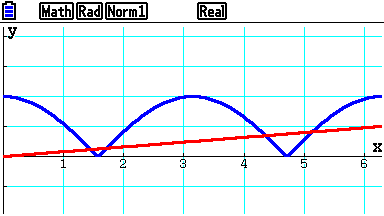
\includegraphics[width=0.4\textwidth]{./assets/5bi.png}
                              \end{center}

                        \item Hence, using the same axes, sketch a suitable straight line to determine the
                              number of solutions for the equation $4 \pi|\cos x|-x=0$ for $0 \leqslant x
                                  \leqslant 2 \pi$. State the number of solutions.

                              \sol{}
                              \begin{align*}
                                  4 \pi|\cos x| & = x              \\
                                  2|\cos x|     & = \frac{x}{2\pi}
                              \end{align*}
                              From the graph, the straight line intersects the curve at 4 points. Therefore, the number of solutions is 4.
                    \end{enumerate}
          \end{enumerate}

    \item Diagram 1 shows the sector $A O B$ of a circle with centre $O$ such that
          $\angle A O B$ is an acute angle. Given the perimeter and the area of the
          sector $A O B$ are $12 \mathrm{~cm}$ and $5 \mathrm{~cm}^2$ respectively.
          \begin{center}
              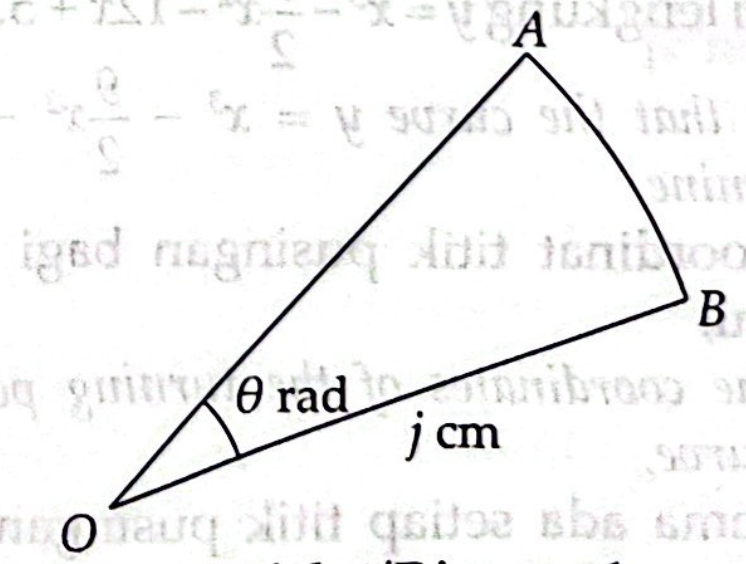
\includegraphics[width=0.3\textwidth]{./assets/6.png}
          \end{center}
          \begin{enumerate}
              \item Form two equations that relate $j$ and $\theta$ based on the above information.

                    \sol{}
                    \begin{align*}
                        \text{Perimeter} & = 2j + \theta j = 12\ \cdots\ (1) \\
                        \text{Area}      & = \frac{1}{2} \theta j^2 = 5      \\
                        \theta j^2       & = 10                              \\
                        \theta           & = \frac{10}{j^2}\ \cdots\ (2)
                    \end{align*}

                    \newpage
              \item Hence, find the value of $j$ and of $\theta$.

                    \sol{}
                    Substituting equation $(2)$ into equation $(1)$,
                    \begin{align*}
                        2j + \frac{10}{j^2} \cdot j & = 12                                \\
                        2j + \frac{10}{j}           & = 12                                \\
                        2j^2 + 10                   & = 12j                               \\
                        2j^2 - 12j + 10             & = 0                                 \\
                        j^2 - 6j + 5                & = 0                                 \\
                        (j-5)(j-1)                  & = 0                                 \\
                        j = 5\                      & \text{or}\ j = 1\ (\text{rejected}) \\
                        \theta                      & = \frac{10}{5^2} = \frac{10}{25}    \\
                                                    & = \frac{2}{5}                       \\
                                                    & = 0.4 \text{ rad}
                    \end{align*}
                    Therefore, $j=5$ and $\theta=0.4$ rad.
          \end{enumerate}

    \item \begin{enumerate}
              \item Determine the number of ways to form 4-digit odd numbers from the digits 4, 5,
                    7 and 9 if the number must be less than 7000.

                    \sol{}

                    First, choose the thousands place. Since the number must be less than 7000, the
                    thousands place can only be 4 or 5.

                    If the thousands place is 4, then the units place can be filled in 3 ways.

                    If the thousands place is 5, then the units place can be filled in 2 ways.

                    The tens and hundreds place can be filled in $\permtwo[2]{2} = 2$ ways.

                    The total number of ways to form the 4-digit odd numbers is $(3+2)2 = 10$.

              \item Diagram 2 shows a normal distribution graph which is symmetrical at $X=32$.

                    \begin{center}
                        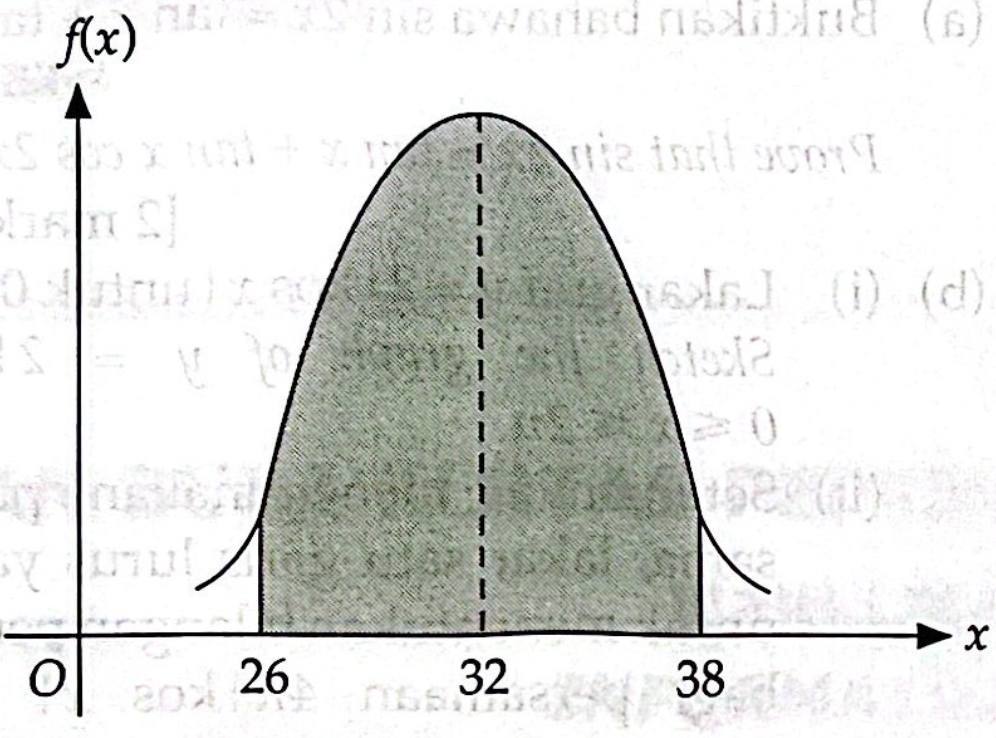
\includegraphics[width=0.4\textwidth]{./assets/7b.png}
                    \end{center}
                    \begin{enumerate}
                        \item State the mean, $\mu$.

                              \sol{}

                              The mean, $\mu = 32$.

                              \newpage

                        \item Express the shaded region in probability notation.

                              \sol{}

                              The shaded region is $P(26<X<38)$.

                        \item If the probability of the shaded region is 0.68 , find $P(X<26)$.

                              \sol{}
                              \begin{align*}
                                  P(X<26) & = 0.5 - \frac{0.68}{2} \\
                                          & = 0.5 - 0.34           \\
                                          & = 0.16
                              \end{align*}
                    \end{enumerate}
          \end{enumerate}

    \item \begin{enumerate}
              \item Find the equation of the tangent and normal to the curve $f(x)=x^3-3 x^2+6$ at
                    point $A(3,6)$.

                    \sol{}
                    \begin{align*}
                        f'(x) & = 3x^2 - 6x     \\
                        f'(3) & = 3(3)^2 - 6(3) \\
                              & = 27 - 18       \\
                              & = 9
                    \end{align*}
                    The gradient of the tangent is 9. The equation of the tangent is
                    \begin{align*}
                        y-6 & = 9(x-3)  \\
                        y   & = 9x-27+6 \\
                        y   & = 9x-21
                    \end{align*}
                    The gradient of the normal is $-\dfrac{1}{9}$. The equation of the normal is
                    \begin{align*}
                        y-6 & = -\frac{1}{9}(x-3)           \\
                        y   & = -\frac{1}{9}x+\frac{1}{3}+6 \\
                        y   & = -\frac{1}{9}x+\frac{19}{3}
                    \end{align*}

              \item Given that the curve $y=x^3-\dfrac{9}{2} x^2-12 x+5$. Determine
                    \begin{enumerate}
                        \item the coordinates of the turning point of the curve,

                              \sol{}
                              \begin{align*}
                                  y'           & = 3x^2 - 9x - 12 = 0   \\
                                  x^2 - 3x - 4 & = 0                    \\
                                  (x-4)(x+1)   & = 0                    \\
                                  x            & = 4\ \text{or}\ x = -1
                              \end{align*}
                              When $x=4$, $y=4^3-\dfrac{9}{2}(4)^2-12(4)+5=-51$. \\
                              When $x=-1$, $y=(-1)^3-\dfrac{9}{2}(-1)^2-12(-1)+5=\dfrac{23}{2}$. \\
                              The coordinates of the turning points are $(4,-51)$ and $\left(-1,\dfrac{23}{2}\right)$.

                        \item whether each turning point is a maximum or minimum point.

                              \sol{}
                              \begin{align*}
                                  y''(x)  & = 6x - 9          \\
                                  y''(4)  & = 6(4) - 9 = 15   \\
                                  y''(-1) & = 6(-1) - 9 = -15
                              \end{align*}
                              The turning point $(4,-51)$ is a minimum point and the turning point $\left(-1,\dfrac{23}{2}\right)$ is a maximum point.

                    \end{enumerate}
          \end{enumerate}
    \item Use graph paper to answer this question.

          Table 1 shows the values of two variables, $x$ and $y$, obtained from an
          experiment. The variables $x$ and $y$ are related by the equation $p y=x^2+q
              x$, where $p$ and $q$ are constants.

          \begin{center}
              \begin{tabular}{|c|c|c|c|c|c|c|}
                  \hline$x$ & 1 & 2 & 3 & 4  & 5  & 6  \\
                  \hline$y$ & 2 & 5 & 9 & 14 & 20 & 27 \\
                  \hline
              \end{tabular}
          \end{center}

          \begin{enumerate}
              \item Plot $\dfrac{y}{x}$ against $x$ by using a scale of $2 \mathrm{~cm}$ to 1 unit
                    on the $x$-axis and $2 \mathrm{~cm}$ to 0.5 unit on the $\dfrac{y}{x}$-axis.
                    Hence, draw the line of best fit.
              \item Using the graph in $9(a)$, find the value of
                    \begin{enumerate}
                        \item $p$,
                        \item $q$.
                    \end{enumerate}
          \end{enumerate}

    \item Diagram 3 shows a straight line $A B$ which intersects a straight line $B C$ at
          point $B$. The point $C$ lies on the $y$-axis.
          \begin{enumerate}
              \item Find
                    \begin{enumerate}
                        \item the equation of the straight line $A B$,
                        \item the coordinates of point $B$.
                    \end{enumerate}

              \item The straight line $A B$ is extended to point $D$ such that $A B: B D=1: 3$.
                    Find the coordinates of point $D$.
              \item Point $P$ moves such that its distance from point $A$ is always 5 units. Find
                    the equation of the locus of point $P$.

              \item Determine whether point $(2,6)$ lies in the locus of point $P$.
          \end{enumerate}
    \item \begin{enumerate}
              \item Find the range of values of $x$ if $(x-2)^2>16-3 x$.
              \item Diagram 4 shows the curve of a quadratic function $f(x)=x^2+m x+8$. The curve
                    has a minimum point $B(3, h)$ and intersects the $f(x)$-axis at point $A$.
                    \begin{enumerate}
                        \item Find the coordinates of point $A$.
                        \item By using the method of completing the square, find the value of $m$ and of $h$. \item Determine the range of values of $x$ if $f(x)<8$.
                    \end{enumerate}
          \end{enumerate}
\end{enumerate}
\end{document}